% !TeX spellcheck = en_US
\documentclass[aspectratio=1610]{beamer}
\mode<presentation>
{
  \usetheme{Boadilla}
  \setbeamercovered{transparent}
  
  \definecolor{cobalt}{rgb}{0.0, 0.20, 0.50}
  
  \usecolortheme[named=cobalt]{structure}
  %\usecolortheme{lily}
  %\setbeamercolor{headline}{fg=cyan!80!black}
  % \setbeamercolor{frametitle}{bg=white}.
}

\makeatletter
\define@key{beamerframe}{wide}[10pt]{%
	\def\beamer@cramped{\itemsep #1\topsep0.5pt\relax}}
\makeatother
	

\usepackage[english]{babel}
\usepackage[utf8]{inputenc}
\usepackage{times}
\usepackage[T1]{fontenc}
\usepackage{array}
\usepackage{xcolor}
\usepackage{colortbl}
\usepackage{booktabs}

\title[Winter - Lecture 1] % (optional, use only with long paper titles)
{Macroeconomic Theory and Policy: Lecture  W1 (Ch.7 and Ch.8)}

\author[University of Toronto] % (optional, use only with lots of authors)
{}
\date[] % (optional, should be abbreviation of conference name)

\begin{document}

\begin{frame}
  \titlepage
\end{frame}

\begin{frame}[wide]{What are You Going to Learn (Ch. 7)}
	\begin{itemize}
		\item Some fact about labour data
%		\item How a supply-and-demand model helps us understand the labor market
		\item How labor market distortions like taxes and firing costs affect employment in the long run
%		\item How to compute present discounted values
%		\item Why the return to a college education has risen enormously over the last half-century
	\end{itemize}
\end{frame}

\begin{frame}[wide]{The U.S. Labor Market}
	\begin{itemize}
		\item In the U.S. labor market (similar for Canada),
		\begin{itemize}
			\item Wages account for two-thirds of per capita GDP
			\item Average wages have grown 2 percent per year for the last century 
			\begin{itemize}
				\item Roughtly the same as the GDP growth
				\item But, not all are growing at the same rate
			\end{itemize}
		\end{itemize}
		\vspace{2mm}
		\item The employment-population ratio:
		\begin{itemize}
			\item Fraction of the civilian population over the age of 16 that is working
			\item Has been increasing over time
			\item Decreases during recessions
			
		\end{itemize}
	\end{itemize}
\end{frame}

\begin{frame}[wide]{Ratio of Employment to Population in the United States, 1960–2016}
	\begin{itemize}
		\item Over the last 50 years, the employment-population ratio has been increasing (peak around 65\%)
		\begin{itemize}
			\item Mostly due to the increase in female workers participation
		\end{itemize}
		\item Decline during recession in particular during 2007-2009 and other recession
	\end{itemize}
	\begin{figure}
		\centering
		\includegraphics[width=0.5\linewidth]{"Figures/MACRO6_FIG07.01"}
	\end{figure}
	
\end{frame}

\begin{frame}[wide]{Ratio of Employment to Population in the Canada, 1976–2021}
	\begin{itemize}
		\item Canada's number is similar to that of the US
		\item The notable difference is that the ratio was still rising during the US recession in year 2000 
	\end{itemize}
	\begin{figure}
		\centering
		\includegraphics[width=0.5\linewidth]{"Figures/Employment to Population in the Canada"}
	\end{figure}
	\footnotetext{Source: Organization for Economic Co-operation and Development, Employed Population: Aged 15 and over: All Persons for Canada [LFEMTTTTCAM647S], retrieved from FRED, Federal Reserve Bank of St. Louis; https://fred.stlouisfed.org/series/LFEMTTTTCAM647S.}
\end{frame}

\begin{frame}[wide]{The Composition of the U.S. Labor Force, February 2016}
	\begin{itemize}
		\item A person is unemployed if (i) does not have a job, (ii) has actively searched for a job in the last 4 weeks, and (iii) Is available for work
	\end{itemize}
	\begin{figure}
		\centering
		\includegraphics[width=0.6\linewidth]{"Figures/Composition of the U.S. Labor Force, February 2016"}
	\end{figure}
\end{frame}

\begin{frame}[wide]{The U.S. Labour Market}
	\begin{itemize}
		\item The unemployment rate: the fraction of the labor force that is unemployed
		\[\text{Unemployment Rate } = \frac{\text{Unemployed}}{\text{Labour Force}} \times 100\]
		\item The unemployment rate is another common measure for analyzing the state of the labor market
		\item There are different types of unemployment: Frictional, Structural and	Cyclical 
		\begin{itemize}
			\item We will cover them later
		\end{itemize}
		\item There are a few alternative measure of unemployment, but most of them are highly correlated
	\end{itemize}
\end{frame}

\begin{frame}[wide]{The U.S. Unemployment Rate}
	\begin{figure}
		\centering
		\includegraphics[width=0.6\linewidth]{"Figures/MACRO6_FIG07.02"}
	\end{figure}
	
\end{frame}

\begin{frame}[wide]{The Dynamics of the Labor Market}
	\begin{itemize}
		\item For most people, periods of unemployment are relatively short
		\vspace{1mm}
		\begin{itemize}
			\item Each month, about 25 percent of people who are unemployed will find a job
		\end{itemize}
		\item However, a significant fraction remain unemployed for long periods of time
		\vspace{1mm}
%		\item Many countries have developed social safety nets (Employment Insurance, etc)
%		\begin{itemize}
%			\item Difficult to determine if this is a causal relationship
%		\end{itemize}
	\begin{figure}
		\centering
		\includegraphics[width=0.9\linewidth]{"Figures/long-term unemployment"}
	\end{figure}
		\item Job creation and job destruction occur each month
		\begin{itemize}
			\item Some workers would be hired, while some quit their job or got fired
			\item Happen during both expansionary period or recession
		\end{itemize}
	\end{itemize}
	
\end{frame}

%\begin{frame}[wide]{The U.S. Long-term Unemployment Rate}
%	
%	
%\end{frame}

%\begin{frame}[wide]{Supply and Demand of Labour Market}
%	\begin{itemize}
%		\item Downward-sloping labour demand
%		\begin{itemize}
%			\item The demand side in the labour is the firm
%			\item Diminishing marginal product of labour (MPL) -- Firms hire workers until MPL equals wage rate
%		\end{itemize}
%		\item Upward-sloping labour supply curve
%		\begin{itemize}
%			\item Price of leisure is higher when wages are higher
%			\item Substitution effect outweighs the income effect for all levels of wages
%		\end{itemize}
%		\item The intersection of labour supply and demand determines the
%		\begin{itemize}
%			\item level of employment
%			\item wage rate
%		\end{itemize}
%		
%	\end{itemize}
%\end{frame}
%
%\begin{frame}[wide]{Supply and Demand of Labour Market}
%	\begin{itemize}
%		\item The labour market clears at the wage w and level of employment L
%		\item The amount of labour supplied by workers equals the amount demanded by firms in a competitive market
%		
%	\end{itemize}
%	\begin{figure}
%		\centering
%		\includegraphics[width=0.5\linewidth]{"Figures/demand and supply labour market"}
%	\end{figure}
%	
%\end{frame}
%
%\begin{frame}[wide]{A Change in Labour Supply}
%	\begin{itemize}
%		\item If the government collects a tax on wages
%		\begin{itemize}
%			\item A worker receives less money for each labour provided and supplies less labour—this applies to any wage
%			\item The labour supply curve shifts left/upward
%			\item To be in equilibrium, firms must raise wages
%		\end{itemize}
%	\end{itemize}
%\end{frame}
%
%\begin{frame}[wide]{An Income Tax at Rate $\tau$}
%	\begin{itemize}
%		\item The labour supply curve shifts up -- for any given wage w that the firm pays, the worker receives less, and therefore supplies less labour
%		\item This reduction in labour supply  raises the wage the firm has to pay to $w'$ and 		reduces the level of employment to $L'$ 
%	\end{itemize}
%	\begin{figure}
%		\centering
%		\includegraphics[width=0.5\linewidth]{"Figures/demand and supply labour market1"}
%	\end{figure}
%	
%\end{frame}
%
%\begin{frame}[wide]{A Change in Labour Demand}
%	\begin{itemize}
%		\item Several factors can lead to a reduction in labour demand, an example is an increase in the price of an input
%		\item It can also be when the government creates regulations making it harder to fire workers, it will increase cost for the firm and firms will demand fewer workers
%		\begin{itemize}
%			\item Firms are subject to risk of information (is the labour a good worker or not?) or risk of business cycle
%			\item Labour demand shifts left. As a results, 	wages and employment fall
%		\end{itemize}
%		
%		\item As discouraged workers drop out of the labour force, this reduces the numerator and the denominator of the unemployment rate, causing the unemployment rate to fall
%		\begin{itemize}
%			\item However, we should be careful regarding our interpretation of this statistic
%			\item This is not necessarily a sign of labour market improvement
%		\end{itemize}
%		
%	\end{itemize}
%\end{frame}
%
%\begin{frame}[wide]{A Reduction in Labour Demand}
%	\begin{itemize}
%		\item The wage falls to $w'$ and employment falls to $L'$, the economy moves from its starting point A to the new equilibrium point B
%		\item The employment-population ratio therefore also declines
%		\item Unemployment rate to rise initially in this case, and then perhaps to recover as discouraged workers drop out of the labour force
%	\end{itemize}
%	\begin{figure}
%		\centering
%		\includegraphics[width=0.4\linewidth]{"Figures/demand and supply labour market2"}
%	\end{figure}
%	
%\end{frame}
%
%\begin{frame}[wide]{Wage Rigidity}
%	\begin{itemize}
%		\item Wage rigidity: wages fail to adjust after a shock to labour demand or supply
%		\begin{itemize}
%			\item Usually, the rigidity happens when wage fall, but not when wage rise
%		\end{itemize}
%		\item What happens if wages do not fall in the above demand shock example?
%		\begin{itemize}
%			\item The labour market will not clear; this results in a larger fall in employment
%		\end{itemize}
%	\end{itemize}
%\end{frame}
%
%\begin{frame}[wide]{A Reduction in Labour Demand with Wage Rigidity}
%	\begin{itemize}
%		\item Wage fixed at $\bar{w}$ initially
%		\item Can result in an even larger reduction in employment (compare points B and C)
%		\item Important in the short run
%	\end{itemize}
%	\begin{figure}
%		\centering
%		\includegraphics[width=0.55\linewidth]{"Figures/demand and supply labour market3"}
%	\end{figure}
%	
%\end{frame}
%
%\begin{frame}[wide]{Case Study: Supply and Demand Shocks in the U.S. Labour Market}
%	\begin{itemize}
%		\item Rise in employment-population ratio, mainly due to an increase in female workers
%		\vspace{1mm}
%		\begin{itemize}
%			\item Supply shocks: Changes in social norms
%			\item Demand shock:	Changes in work culture that was against women
%			\item Goldin (2014) shows that the male-female wage has been converging 
%		\end{itemize}
%		\begin{figure}
%			\centering
%			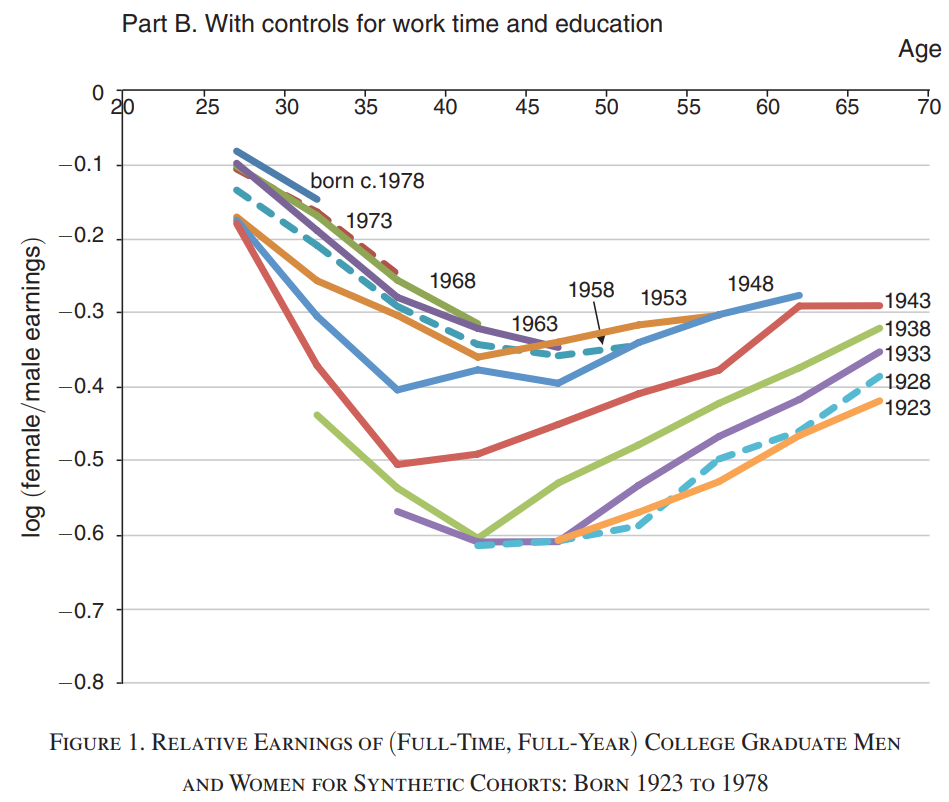
\includegraphics[width=0.45\linewidth]{Figures/female-male-wage-converge}
%		\end{figure}
%	\end{itemize}
%	\footnotetext{Goldin C. A Grand Gender Convergence: Its Last Chapter. American Economic Review. 2014;104 (4)}
%\end{frame}
%
%\begin{frame}[wide]{Case Study: Supply and Demand Shocks in the U.S. Labour Market}
%	\begin{itemize}
%		\item Rising unemployment in the 1960s and 1970s 
%		\item Robert Shimer suggests that it may due to Baby-boomer generation entering the workforce 
%		\vspace{1mm}
%		\begin{itemize}
%			\item Because teenage and young-adult unemployment rates are much higher than those for middle-aged workers, the entry of baby boomers into the labour force in the 1960s and 1970s raised the unemployment rate by about two percentage points
%			\item However, as these individuals gained experience, their individual unemployment rates declined
%			\item This maturing explains about 1.5 percentage points of the decline in unemployment in the 1980s and 1990s
%			%\item Supply shock:	Younger workers have higher unemployment rates
%		\end{itemize} 
%		
%	\end{itemize}
%\end{frame}

\begin{frame}[wide]{Different Kinds of Unemployment}
	\begin{itemize}
		\item Cyclical unemployment: Associated with short-run fluctuations in output
		\vspace{1mm}
		\begin{itemize}
			\item Due to business cycle
			\item Measure as the difference between actual rate and natural rate
		\end{itemize}
		\item The natural rate of unemployment:	Rate that would prevail with no cyclical unemployment
		\vspace{1mm}
		\begin{itemize}
			\item Frictional unemployment: Workers between jobs in the dynamic economy
			\begin{itemize}
				\item e.g., Instead of accepting the first available job, workers take time to match their skills with demands of firms, etc
			\end{itemize}
			\item Structural unemployment: labour market failure to match workers and firms
			\begin{itemize}
				\item e.g., Hiring and firing costs, the level of unemployment benefits, the level of the minimum wage, etc
				
			\end{itemize}
		\end{itemize}
		
	\end{itemize}
\end{frame}

\begin{frame}[wide]{Bathtub Model of Unemployment}
	\begin{itemize}
		\item Recall that job separation and matching happen  at the same time
		\item Bathtub model: States how employment and unemployment evolve over time
		\[E_t + U_t = \bar{L}\]
		where
		\item[] $E_t$: Employment
		\item[] $U_t$: Unemployment
		\item[] $\bar{L}$: Size of Labour Force
		\item $E_t$ and $U_t$ are endogenous variables while $\bar{L}$ is a constant
	\end{itemize}
\end{frame}

\begin{frame}[wide]{Bathtub Model of Unemployment}
	\begin{itemize}
		\item Unemployment changes over time by following:
		\[\Delta U_{t+1} = \bar{s}E_t - \bar{f} U_t\]
		where
		\begin{itemize}
			\item[] $\Delta U_{t+1}$ is the change in employment
			\item[] $\bar{s}$ is the job separation rate
			\item[] $\bar{f}$ is the job-finding rate
		\end{itemize}
		\item The term $ \bar{s}E_t$ is the number of employed people who lose their jobs
		\item The term $ \bar{f} U_t$ is the number of unemployed people who find new jobs
		\item The value for $\bar{s}$ is usually around value 1.4\%  per month
	\end{itemize}
\end{frame}

\begin{frame}[wide]{Bathtub Model of Unemployment}
	\begin{itemize}
		\item The bathtub model has a steady state -- the number of people employed and unemployed is constant
		\begin{itemize}
			\item Occurs when the change in unemployment is zero
			\item The number of people losing jobs exactly equals the number of people finding new jobs
		\end{itemize}
		\item Set the change in unemployment ($\Delta U_{t+1}$) to zero and sub in the unemployment def
		\[0=\bar{s} E_t - \bar{f} U_t = \bar{s} (\bar{L} -U_t) - \bar{f} U_t = \bar{s}\bar{L} - (\bar{s}+\bar{f}) U_t\]
		\item Solving for $U_t$
		\[U_t = \frac{\bar{s}\bar{L}}{\bar{s}+\bar{f}}\]
	\end{itemize}
\end{frame}

\begin{frame}[wide]{Bathtub Model of Unemployment}
	\begin{itemize}
		\item The unemployment rate is then
		\vspace{2mm}
		\[u^* = \frac{U^*}{\bar{L}} = \frac{\bar{s}}{\bar{s} + \bar{f}}\]
		\vspace{2mm}
		\item This unemployment rate holds in the steady state (i.e., long run), this would be the natural rate of unemployment in the Bathtub Model
		\vspace{2mm}
		\item To alter the natural rate of unemployment:
		\begin{itemize}
			\item Change the job-finding rate, $\bar{f}$
			\item Change the job separation rate, $\bar{s}$
		\end{itemize}
	\end{itemize}
\end{frame}

\begin{frame}[wide]{Bathtub Model of Unemployment}
	\begin{itemize}
		\item Some policies may have alter the unemployment rate. 	For example, one may try to reduce the job separation rate by imposing firing costs on firms: 
		\vspace{2mm}
		\begin{itemize}
			\item Any firm that fires a worker must pay one year's salary as a severance payment.
			\item Firms may then become reluctant to hire new workers, reducing the job-finding rate
			\item The net of these effects could be to increase the natural rate of unemployment rather than to decrease it
		\end{itemize}
	\end{itemize}
\end{frame}

\begin{frame}[wide]{Bathtub Model of Unemployment}
	\begin{itemize}
		\item What determine the job finding rate?
		\item Typically, economist model it with a matching function that take vacancy and job search effort as the determinant for job finding (matching) rate
		\item Empirically, vacancy data has been survey by statistic agency (US in 2000 and Canada in 2015)
		\begin{itemize}
			\item There are also works screening through online job posting website (e.g., indeed, monsters, etc)
		\end{itemize}
		\item However, search effort is harder to measure
		\begin{itemize}
			\item The CPS in the US and LFS in the Canada has supplement survey question asking about the job search effort
			\item But researchers find different conclusion regarding its relationship to business cycle because of difference in method
		\end{itemize}
	\end{itemize}
\end{frame}

\begin{frame}[wide]{Job Vacancy}
	\begin{itemize}
		\item The vacancy fall when the economic hit a recession, and recover slowly afterward
		\item Particular high vacancy rate after the pandemic
	\end{itemize}
	\begin{figure}
		\centering
		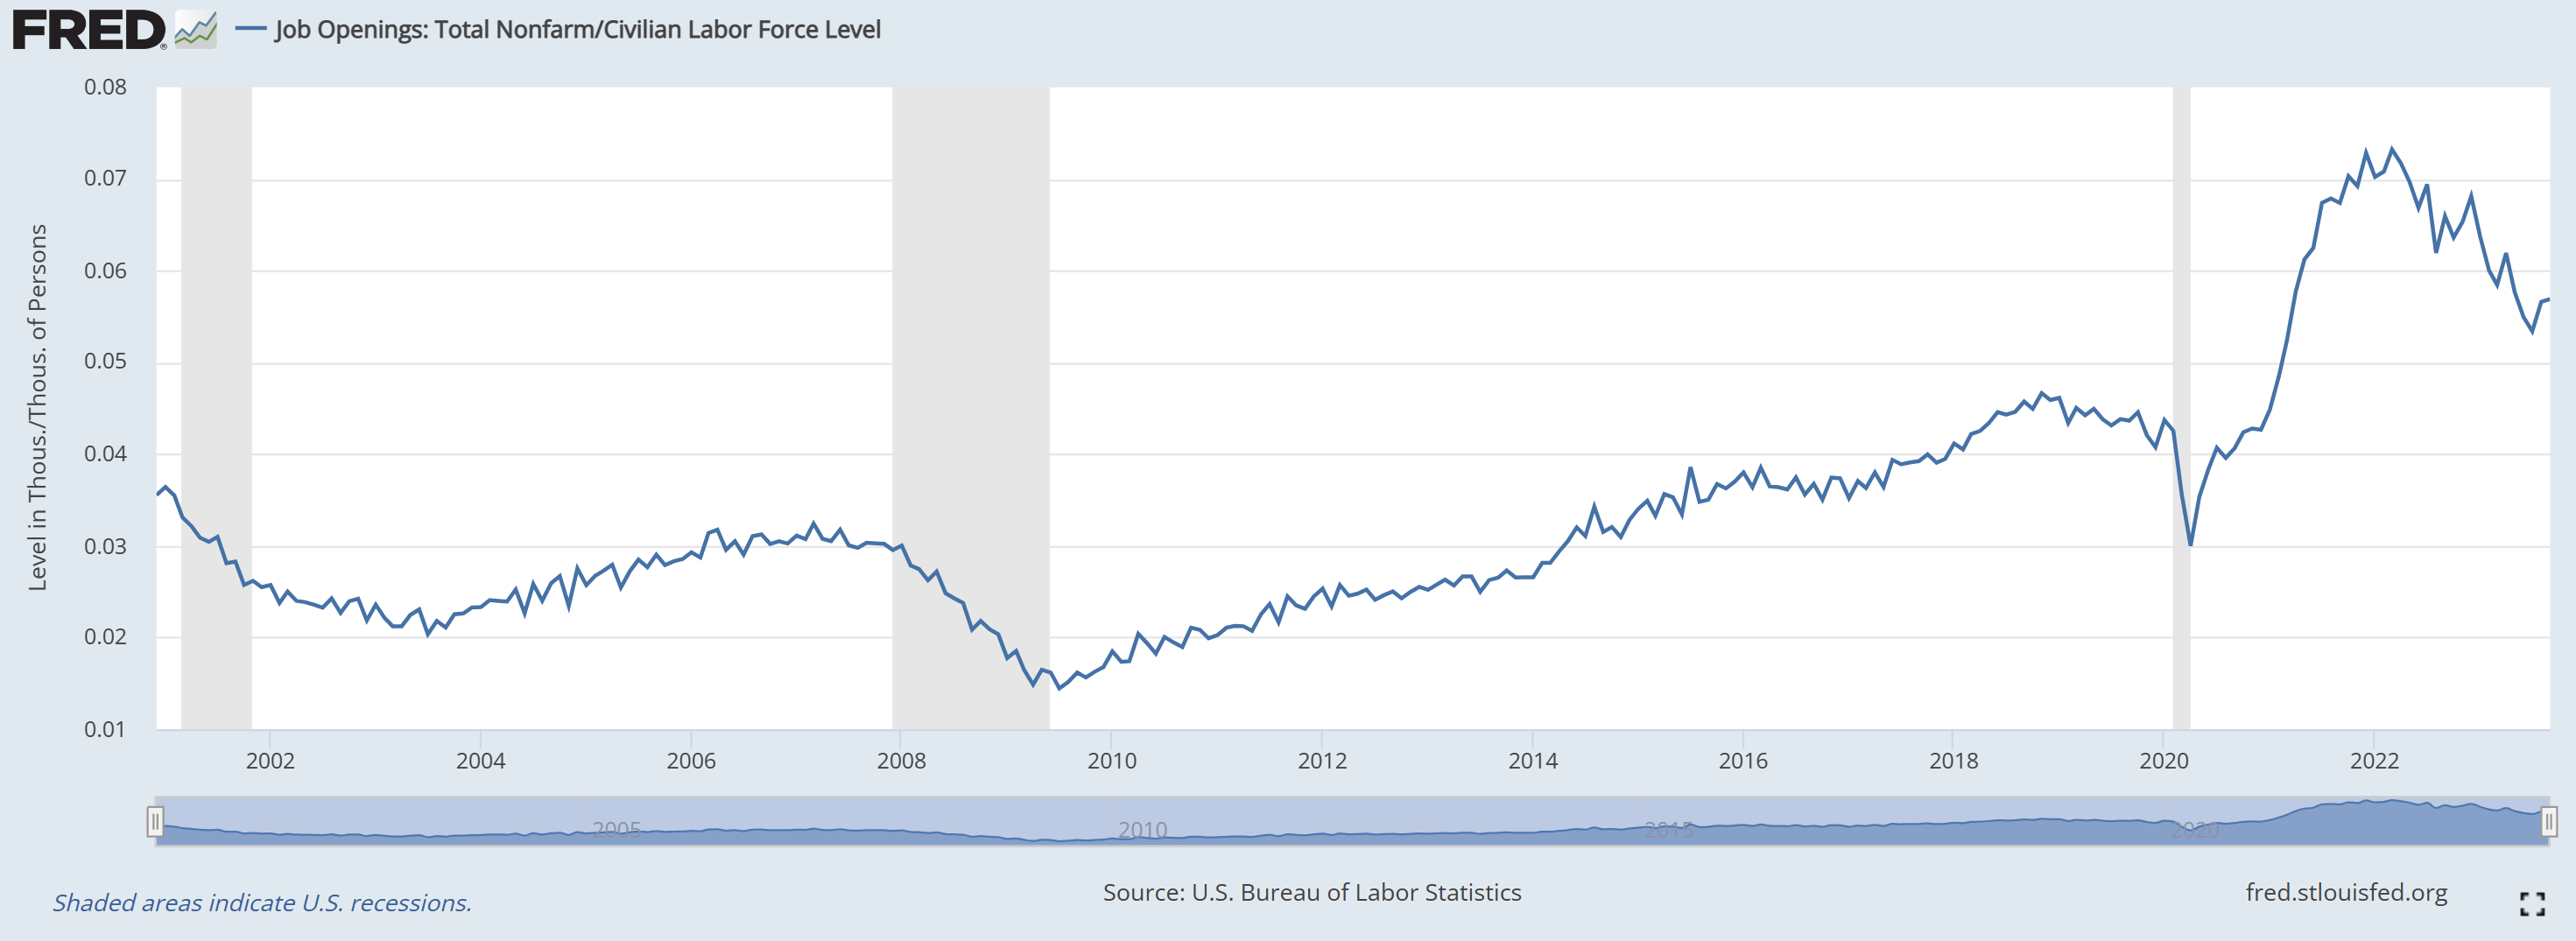
\includegraphics[width=1\linewidth]{Figures/job_vacancy}
	\end{figure}
\end{frame}

%\begin{frame}[wide]{Job Vacancy}
%	\begin{itemize}
%		\item The series is short but shows similar pattern as the overall job vacancy 
%	\end{itemize}
%	\begin{figure}
%		\centering
%		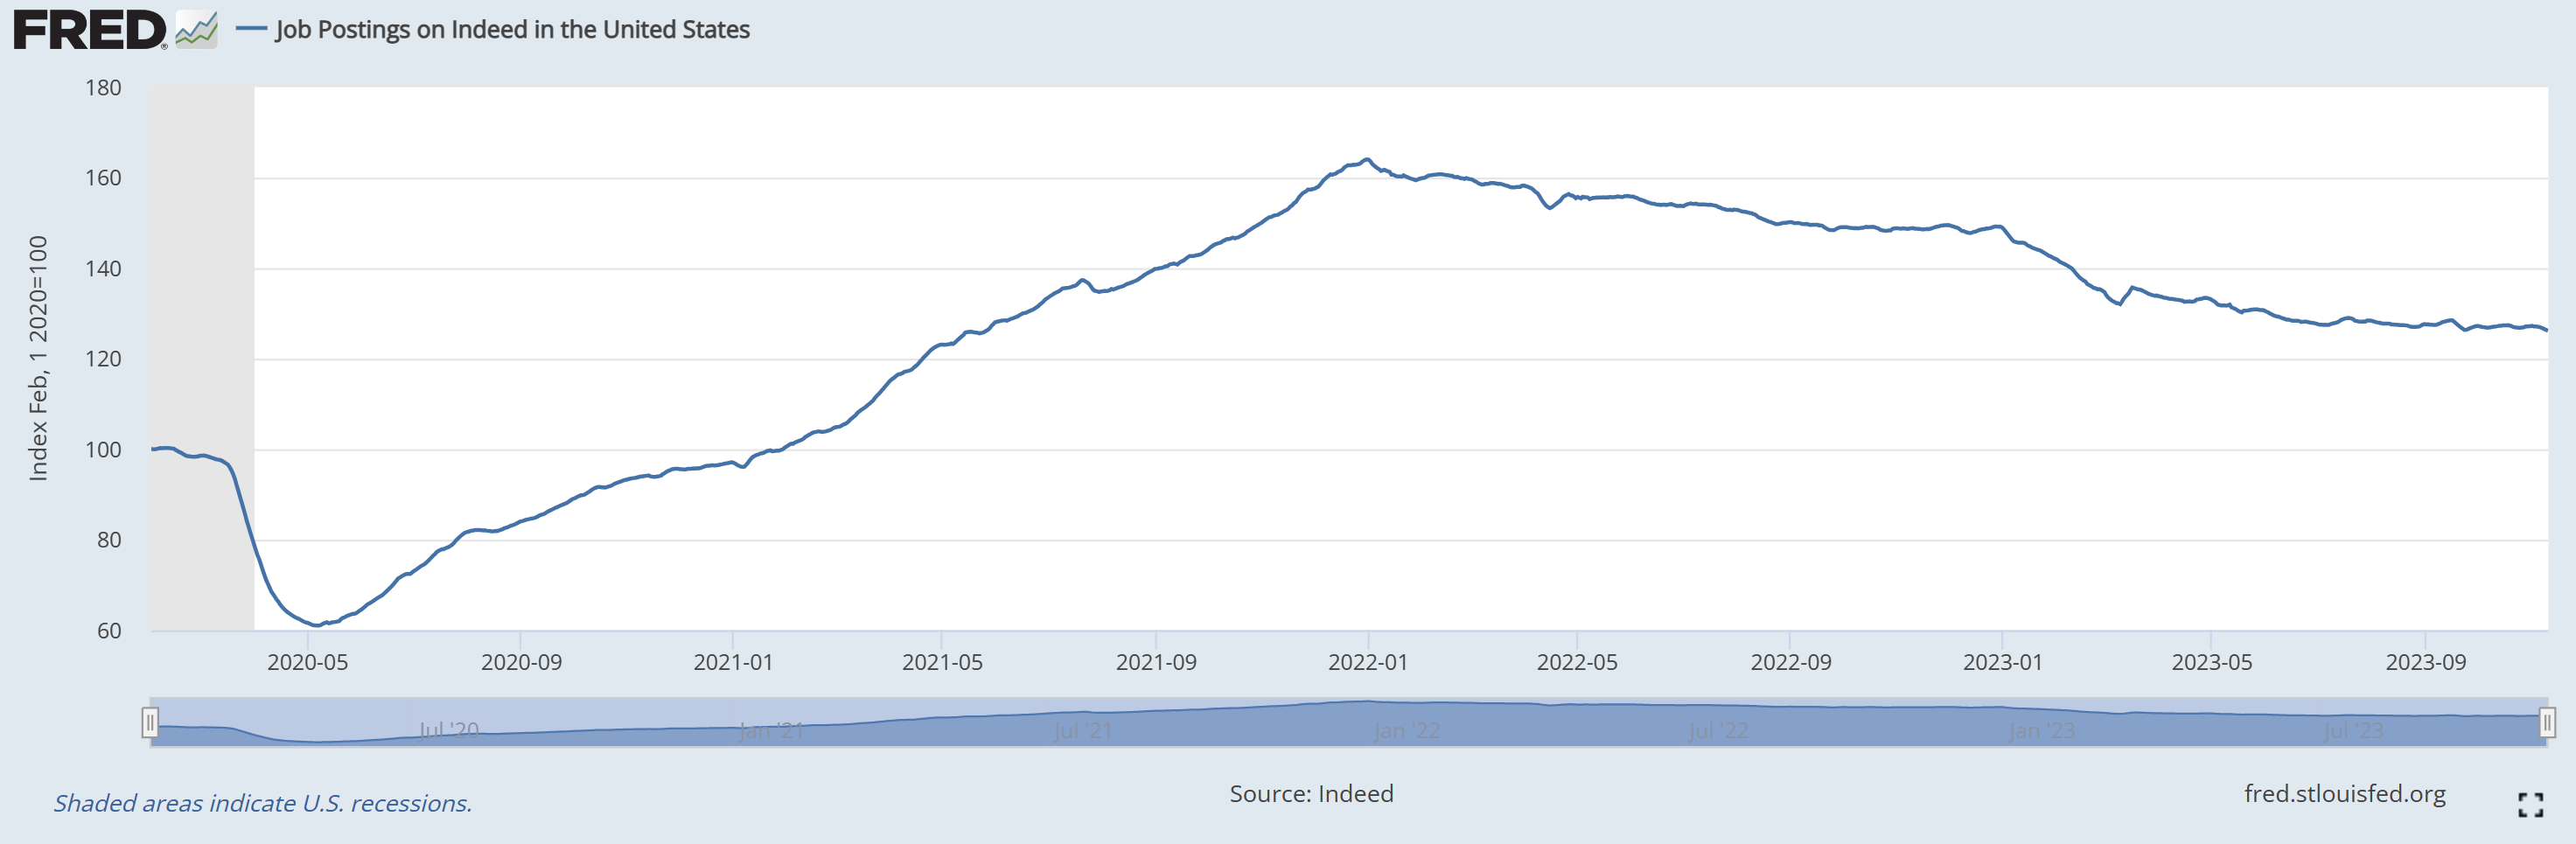
\includegraphics[width=1\linewidth]{Figures/job_vacancy1}
%	\end{figure}
%	
%\end{frame}

%\begin{frame}[wide]{Job Search Effort}
%	\begin{itemize}
%		\item Economists have collect data other than official source
%		\begin{itemize}
%			\item Job search platforms (e.g., Faberman et al, 2019, Marinescu et al, 2021)
%			\item Other survey (NY FED survey) (e.g.,  Faberman et al., 2022)
%		\end{itemize}
%		\item But, data is relatively short. Some economist went back to pre-WWII (e.g., Atalay et al., 2020, Bi et al., 2023)
%		\item Bi et al. (2023) screen through job ad section of various newspapers
%	\end{itemize}
%	\begin{figure}
%		\centering
%		
\includegraphics[width=0.65\linewidth]{Figures/search_effort}
%	\end{figure}
%	
%\end{frame}
%
%\begin{frame}[wide]{Job Search Effort}
%	\begin{itemize}
%		\item Job search effort depends on how many people are unemployed. Looking at the situation wanted index the pattern is unclear
%		\item Bi et al. (2023) divide the situation wanted index by unemployment rate and get the search effort (RHS) and found that search effort is procyclical
%	\end{itemize}
%	\begin{figure}
%		\centering
%		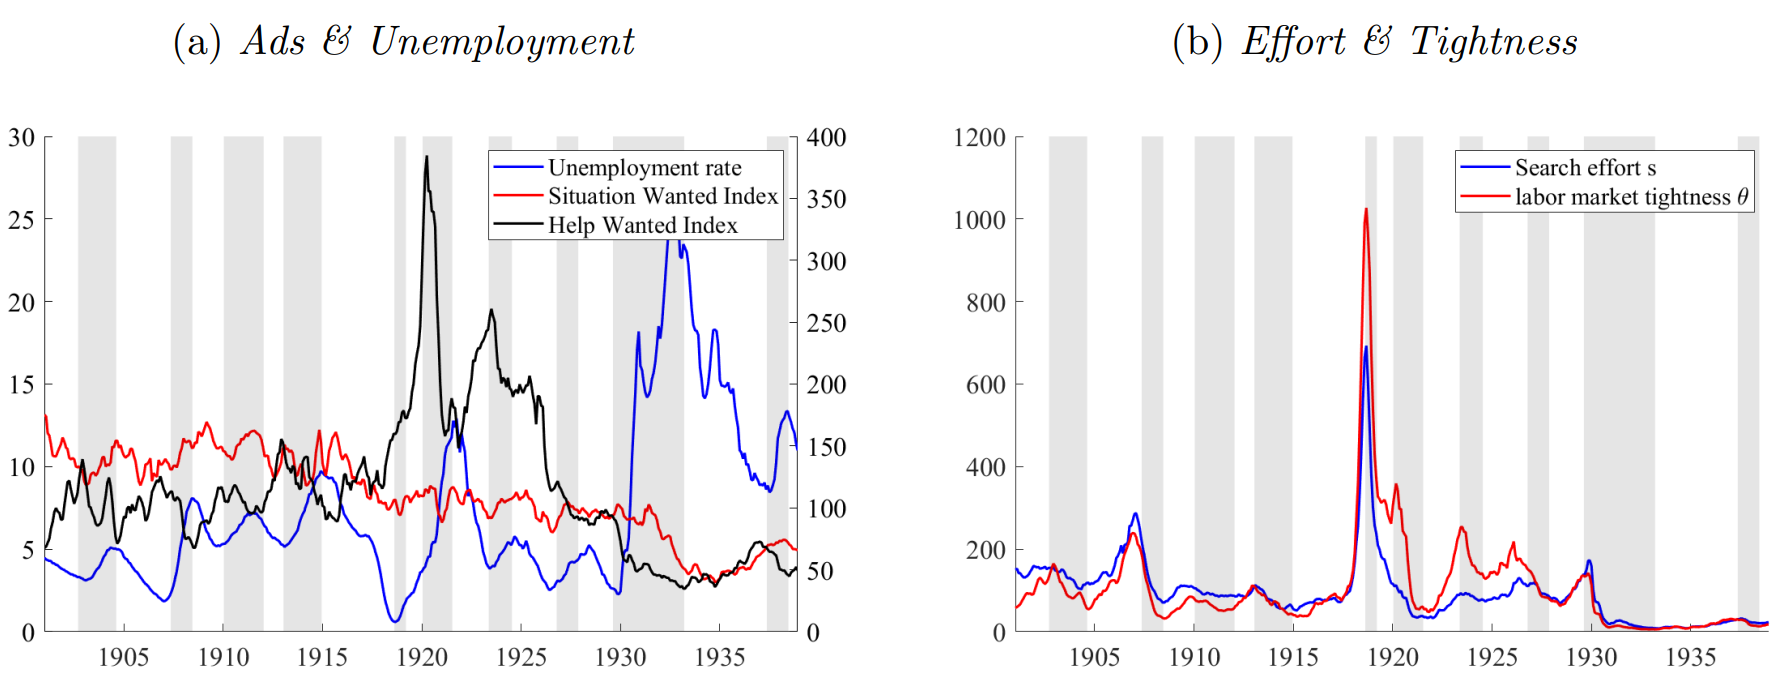
\includegraphics[width=1\linewidth]{Figures/search_effort2}
%	\end{figure}
%\end{frame}

\begin{frame}[wide]{Labour Markets around the World}
	\begin{itemize}
		\item Since 1980: Unemployment in Europe is well above the rate in the United States
		\vspace{2mm}
		\item European unemployment has increased because of
		\vspace{1mm}
		\begin{itemize}
			\item Adverse shocks and high oil prices
			\item Inefficient labour market institutions:
			\vspace{1mm}
			\begin{itemize}
				\item Higher unemployment insurance
				\item Welfare benefits (high implicit tax rate for returning to work)
			\end{itemize}
		\end{itemize}
	\end{itemize}
\end{frame}

\begin{frame}[wide]{Unemployment in the United States, Europe, and Japan}
	\begin{itemize}
		\item Japan’s unemployment rate has been substantially below that in the United States and Europe until recent years
		\item European unemployment has been substantially higher than unemployment in the United States in recent decades
		\item Unemployment in Japan, after being low for many decades, began approaching U.S. levels in the 2000s
	\end{itemize}
	\begin{figure}
		\centering
		\includegraphics[width=0.5\linewidth]{"Figures/Unemployment in the United States, Europe, and Japan"}
	\end{figure}
	
\end{frame}

\begin{frame}[wide]{Hours Worked per Person}
	\begin{itemize}
		\item When we look at labour market, we want to examine the intensive margin (hours worked) and extensive margin (employment)
	\end{itemize}
	\begin{figure}
		\centering
		\includegraphics[width=0.7\linewidth]{"Figures/Hours Worked per Person"}
	\end{figure}
	
\end{frame}

\begin{frame}[wide]{Labour Markets around the World}
	\begin{itemize}
		\item GDP per capita is lower in Europe. Why? People work fewer hours 
		\item If working less is voluntary:
		\begin{itemize}
			\item Europeans enjoy leisure or home production more
			\item Welfare is likely improved
		\end{itemize}
		\item If working less is due to distortions in the labour market:
		\begin{itemize}
			\item This outcome is likely not welfare enhancing
		\end{itemize}
	\end{itemize}
\end{frame}

%\begin{frame}[wide]{The Rising Return to Education}
%	\begin{itemize}
%		\item The ``College Premium" equals extra money earned by an employee due to the fact that he has a college education
%		\item Think about the costs and benefits of college,
%		\begin{itemize}
%			\item Costs:  Forgone wages (opportunity cost), tuition (direct expense)
%			\item Benefits:  Premium, more wages later on
%		\end{itemize}
%		\item The return to a college education is large and has been rising over time
%		
%	\end{itemize}
%\end{frame}
%
%\begin{frame}[wide]{The Rising Return to Education}
%	\begin{itemize}
%		\item The premium to having a college degree:
%		\begin{itemize}
%			\item Has been rising rapidly over the last forty years
%			\item Far outweighs the forgone wages and tuition costs
%		\end{itemize} 
%		\begin{figure}
%			\centering
%			\includegraphics[width=0.7\linewidth]{"Figures/The Rising Return to Education"}
%		\end{figure}
%		
%	\end{itemize}
%\end{frame}
%
%\begin{frame}[wide]{The Rising Return to Education}
%	\begin{itemize}
%		\item In theory, when the college premium increase, the supply of college graduate should increase in the long run. Then, the  college premium would diminish
%		\item That would be true if we ignore the demand side -- there was a skill-biased technical change
%		\item New technologies are more effective at improving productivity of college-educated workers, which lead to an increase in demand
%		\item If the demand shift large enough relative to the shift in supply, wages have increased for college grads
%	\end{itemize}
%\end{frame}
%
%\begin{frame}[wide]{The Rising Return to Education}
%	\begin{figure}
%		\centering
%		\includegraphics[width=0.9\linewidth]{"Figures/Understanding the Rising Return to Education"}
%	\end{figure}
%	
%\end{frame}
%
%\begin{frame}[wide]{Case Study: Income Inequality}
%	\begin{itemize}
%		\item Rising college premium is one cause of rising income inequality
%		\item Early 1900s: 	Most inequality associated with capital income
%		\item Recently:	Most inequality associated with salaries and business income
%		\item Inequality can be a beneficial and problematic:
%		\begin{itemize}
%			\item It maybe reflect high returns to innovation in a more integrated world economy, because a lot of the works are very scalable 
%			\begin{itemize}
%				\item Compare hypothetical economy where the IT boom did not happen, everyone's wage grow by 20\%, while the other economy has the top 1\% grow by 100\% and the rest grow by 30\%
%			\end{itemize}
%			\item The cost would be that the society become more polarized
%		\end{itemize}
%		
%	\end{itemize}
%\end{frame}
%
%\begin{frame}[wide]{Income Inequality in the United States and France}
%	\begin{itemize}
%		\item Both France and the US have high inequality in the early 20th century
%		\item It diverged around 1980s
%	\end{itemize}
%	\begin{figure}
%		\centering
%		\includegraphics[width=0.7\linewidth]{"Figures/Income Inequality in the United States and France"}
%	\end{figure}
%	
%\end{frame}
%
%\begin{frame}[wide]{Income Inequality in the United States and Canada}
%	\begin{itemize}
%		\item Meanwhile, Saez and Veall (2004) finds that the income inequality fall in both US and Canada during the early 20th century then rise around 1980
%	\end{itemize}
%	\begin{figure}
%		\centering
%		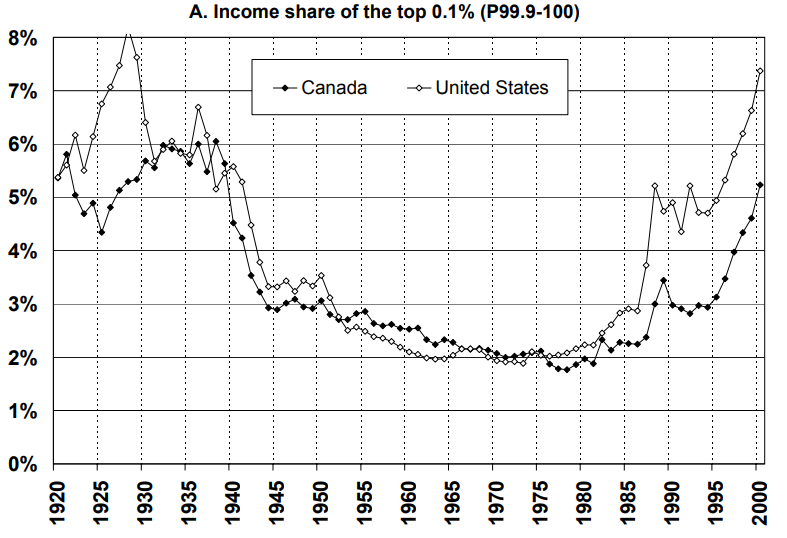
\includegraphics[width=0.5\linewidth]{Figures/canadarevised}
%	\end{figure}
%	\footnotetext{Saez, Emmanuel, and Michael R. Veall. "The evolution of high incomes in Northern America: lessons from Canadian evidence." American economic review 95, no. 3 (2005): 831-849.}
%\end{frame}
%
%\begin{frame}[wide]{Economic Growth and Income Inequality}
%	\begin{itemize}
%		\item So far, we have explored growth as an average income per person 
%		\item Evidence suggests that economic growth may not be equally distributed
%		\item In recent decades, it appears that the top of the income distribution has done better than the bottom
%		\item For longer period perspective, economists also look at the inter-generation income mobility
%		\begin{itemize}
%			\item e.g., how likely a children of a low-middle income earning family can become the top 1\%
%			\item The finding so far is that there is strong correlation between parent income and their children's income, but the chance for breaking into higher income percentile is not low
%		\end{itemize}
%	\end{itemize}
%\end{frame}
%
%\begin{frame}[wide]{Economic Growth and Income Inequality}
%	\begin{itemize}
%		\item In 1980, poor and middle class catching up to the upper class: below the 40th percentile, growth was even faster, and above the 80th percentile growth was slightly slower
%		\item In 2014, the poor and middle class saw slower growth, while the rich experienced faster growth
%	\end{itemize}
%	\begin{figure}
%		\centering
%		\includegraphics[width=0.5\linewidth]{"Figures/Economic Growth and Income Inequality"}
%	\end{figure}
%	
%\end{frame}

\begin{frame}[wide]{What are You Going to Learn (Ch. 8)}
	\begin{itemize}
		\item Understand the nature and costs of inflation. Explore the insights provided by the quantity \item Theory of money and the classical dichotomy into the phenomenon of inflation
		\item Examine the connection between interest rates and inflation using the Fisher equation
		\item Recognize the crucial association between fiscal policy and the occurrence of high inflation.
	\end{itemize}
\end{frame}

\begin{frame}[wide]{Inflation}
	\begin{itemize}
		\item 	Inflation: 	Percentage change in the overall price level
		\[\text{Inflation rate} = \frac{P_{t+1}-P_t}{P_t}\times 100\]
		where $P_t$ is the price in period $t$
		\item Measured usually based on the Consumer Price Index (CPI)
		\begin{itemize}
			\item CPI: Price index for a bundle of consumer goods
		\end{itemize} 
	\end{itemize}
\end{frame}

\begin{frame}[wide]{Inflation Rate in the United States}
	\begin{itemize}
		\item The inflation was around 2\% in the 60s and after the 80s
		\item However, inflation was highest in 1980 at 13.5 percent
		\begin{itemize}
			\item High inflation created arbitrary transfers of wealth and distorted incentives for 	 investment
			\item Businesses that borrowed to finance investment faced extremely high interest rates
		\end{itemize}
	\end{itemize}
	\begin{figure}
		\centering
		\includegraphics[width=0.5\linewidth]{"Figures/Inflation Rate in the United States"}
	\end{figure}
	
\end{frame}

\begin{frame}[wide]{Inflation Rate in the Canada}
	\begin{itemize}
		\item Canada's experience is similar to that in US
		\item Recent inflation surge is not unseen before 
	\end{itemize}
	\begin{figure}
		\centering
		\includegraphics[width=0.9\linewidth]{"Figures/inflation in Canada"}
	\end{figure}
\end{frame}

\begin{frame}[wide]{Case Study: How Much Is That?}
	\begin{itemize}
		\item 	We can use the CPI to evaluate the value of a good in 1950 in today’s dollars
	\end{itemize}
	\begin{figure}
		\centering
		\includegraphics[width=0.7\linewidth]{"Figures/table 8-1"}
	\end{figure}
	
\end{frame}

\begin{frame}[wide]{Case Study: How Much Is That?}
	\begin{itemize}
		\item In 1950, a gallon of gasoline cost 27 cents, while in 2018 it cost around \$2.50 in the United States 		
		\item To compare, we can find the price of the good in 1950 in 2018 dollars
		\[0.27 \times \frac{100}{9.59} = 2.82 \]
		\item We can also compute the other way around
		\[2.5 \times \frac{9.59}{100} = 0.24 \]
		\item Real difference is not as large as the nominal
		 \begin{itemize}
		 	\item Gasoline was actually more expensive in 1950 than in 2018, contrary to how low the 27 cents a gallon sounds
		 \end{itemize}
	\end{itemize}
\end{frame}

\begin{frame}[wide]{What is Money?}
	\begin{itemize}
		\item 	We often think of money as paper currency
		\item But, historically, money was backed by gold or if we go further back, seashells, rocks, other precious metals, etc
		\item Today, paper currency has value because of government decree (fiat money)
		\begin{itemize}
			\item It is no longer backed by gold or silver
			\item There is a mutual agreement that paper currency will be accepted as payment
			\item Money has value because we expect others will value it and accept it as payment
		\end{itemize}
	\end{itemize}
\end{frame}



\begin{frame}[wide]{The Quantity Equation}
	\begin{itemize}
		\item Connects money/currency ($M_t$) and inflation (change in $P_t$)
		\item Velocity of money (V): the average number of times per year that each piece of paper currency is used in a transaction
		\item The amount of money used in purchases ($M_tV_t$) is equal to nominal GDP ($P_tY_t$)
		\[M_t V_t = P_t Y_t\]
	\end{itemize}
\end{frame}

\begin{frame}[wide]{The Classical Dichotomy and Constant Velocity}
	\begin{itemize}
		\item 	The classical dichotomy: the real and nominal sides of the economy are completely separate in the long run
		\begin{itemize}
			\item Economy 1 is produce 10 units of goods and charge \$50,000
			\item Economy 2 is produce 10 units of goods and charge \$1,000,000
			\item The two economy has the same real economy while the nominal side is different
			\item In the growth model, the variables do not depend on money
		\end{itemize}
		\item In the quantity theory of money:
		\begin{itemize}
			\item Real GDP is assumed as exogenously given, determined by real forces (e.g., saving rate, etc)
			\[Y_t = \bar{Y_t}\]
		\end{itemize}
		
	\end{itemize}
\end{frame}

\begin{frame}[wide]{The Classical Dichotomy and Constant Velocity}
	\begin{itemize}
		\item 	The velocity of money: exogenously given constant and assumed to be constant over time
		\[V_t = \bar{V}\]
		\begin{itemize}
			\item the velocity of the M2 definition of money is approximately constant
			\item So, in the long run, this is not an unreasonable assumption
		\end{itemize}
		\item The money supply: determined by the central bank and is exogenously given
		\[M_t = \bar{M_t}\]
		
	\end{itemize}
\end{frame}

\begin{frame}[wide]{The Quantity Theory of Money}
	\begin{itemize}
		\item 	The model has 4 Equations and 4 Unknowns
		\item The quantity equation
		\[M_tV_t = P_tY_t\]
		\item Real GDP from growth model
		\[Y_t = \bar{Y}\]
		\item Exogenous and constant velocity
		\[V_t = \bar{V}\]
		\item Exogenous money supply 
		\[M_t = \bar{M}\]
		\item Exogenous variables/parameters: $\bar{M_t}$, $\bar{V}$ and $\bar{Y_t}$
	\end{itemize}
\end{frame}

\begin{frame}[wide]{The Quantity Theory for the Price Level}
	\begin{itemize}
		\item 	Plug in all the exogenous variables
		\item Solve for the price level:
			\[P^*_t = \frac{\bar{M_t} \bar{V}}{\bar{Y_t}}\]
		\item Prices will rise as a result of
		\begin{itemize}
			\item Increases in the money supply
			\item Decreases in real GDP
		\end{itemize}
		\item In the long run, the key determinant of the price level is the money supply (if $Y_t$ is determined as in Solow model or Romer model)
	\end{itemize}
\end{frame}

\begin{frame}[wide]{The Quantity Theory for Inflation}
	\begin{itemize}
		\item 	Inflation is the growth of the price, applying the rules of growth rates to the quantity equation 
		\[\bar{g}_M + \bar{g}_V = 	\bar{g}_P +\bar{g}_Y\]
		\item In the long run, $V$ is not changing, thus $\bar{g}_V = 0$
		\item Let $g_P=\pi$
		\[\pi^* = \bar{g}_M -\bar{g}_Y\]
	\end{itemize}
\end{frame}

\begin{frame}[wide]{The Quantity Theory for Inflation}
	\[\pi^* = \bar{g}_M -\bar{g}_Y\]
	\begin{itemize}
		\item Changes in money growth do not change real GDP because of the classical dichotomy
		\item So, the change in money lead to one-for-one to changes in the inflation rate
		\item Based on this model, Central bank has a lot of influence on the price level in the long run
		\item Empirically, this holds up both in U.S. and worldwide data
	\end{itemize}
\end{frame}

\begin{frame}[wide]{Measures of the Money Supply}
	\begin{itemize}
		\item 	The monetary base includes currency and accounts (reserves)
		\begin{itemize}
			\item Banks hold accounts with the economy’s central bank
			\item Banks ensure that they have cash on hand in case of withdrawals
		\end{itemize}
		\item We add less liquid from C to MB to M1 to M2
		\item Most of the money are in form of savings deposits and individual money market accounts
	\end{itemize}
	\begin{figure}
		\centering
		\includegraphics[width=0.6\linewidth]{"Figures/table 8-2"}
	\end{figure}
	
\end{frame}

\begin{frame}[wide]{Money Growth and Inflation in the United States, 1870–2018}
	\begin{itemize}
		\item 	A strong positive relationship between money growth and inflation
	\end{itemize}
	\begin{figure}
		\centering
		\includegraphics[width=0.55\linewidth]{"Figures/MACRO6_FIG08.03"}
	\end{figure}
	
\end{frame}

\begin{frame}[wide]{Money Growth and Inflation around the World, 1990–2017}
	\begin{itemize}
		\item In the lower left corner, many countries have low money growth and low inflation (e.g., US, $\bar{g}_M = 5.4\%$ with $\pi=2.8\%$and Germany $\bar{g}=2.8\%$ with $\pi=1.9\%$)
		\item In the upper right corner, we have Peru, Brazil and so forth
	\end{itemize}
	\begin{figure}
		\centering
		\includegraphics[width=0.5\linewidth]{"Figures/Figure 8.3"}
	\end{figure}
\end{frame}

\begin{frame}[wide]{Revisiting the Classical Dichotomy}
	\begin{itemize}
		\item When all prices in the economy double, relative prices are unchanged
		\item When the relative prices of goods are unchanged, nothing real is affected
		\begin{itemize}
			\item If a country opts to introduce a new currency with two additional zeros at the end, the relative price of, say orange and apple, would remain the same
		\end{itemize}
		\item The neutrality of money says that changes in the money supply	have no real effects on the economy and	affect only prices
		\item Empirically, it holds in the long run
		\item But, does not hold in the short run -- nominal prices do not respond immediately to changes in the money supply
	\end{itemize}
\end{frame}

\begin{frame}[wide]{Real and Nominal Interest Rates}
	\begin{itemize}
		\item The real interest rate is equal to the marginal product of capital and is paid in goods
		\item The nominal interest rate 	is the interest rate on a savings account and is paid in dollars
	\end{itemize}
\end{frame}

\begin{frame}[wide]{The Fisher Equation}
	\begin{itemize}
		\item 	The Fisher equation: 
		\[i \approx R+\pi\]
		
		where
		\begin{itemize}
			\item[] $i$ = nominal interest rate
			\item[] $R$ = real interest rate
			\item[] $\pi$ = inflation rate
		\end{itemize}
		\item The nominal interest rate is generally high when inflation is high
	\end{itemize}
\end{frame}

\begin{frame}[wide]{The Fisher Equation}
	\begin{itemize}
		\item 	We can rearrange the equation
		\[R= i-\pi\]
		\item Empirically, the real interest rate has been negative
		\begin{itemize}
			\item This implies that in the short run the real interest rate need not equal the MPK
		\end{itemize}
		\item It is not a number that would be reported by the news or government
		\begin{itemize}
			\item However, one should consider this metric when doing long-term investment
			\item Say, someone retired on fixed income that give 10\% return. However, if the person's cost of living increase by 10\%, this retiree is losing purchasing power every month
		\end{itemize}
	\end{itemize}
\end{frame}

\begin{frame}[wide]{Real and Nominal Interest Rates in the United States, 1960–2015}
	\begin{itemize}
		\item 	The nominal interest rate is the highest in 1981 at 14 percent when the inflation was its highest in 1980 --	This relationship is described by the Fisher equation
		\item In 2009, the real interest rate actually became larger than the nominal interest rate, due to deflation
		\item The real interest rate can also be negative, happened in the 1970s, 2003, and 2010–2015, when the nominal interest rate was very low
		
	
	\end{itemize}
	\begin{figure}
		\centering
		\includegraphics[width=0.5\linewidth]{"Figures/Figure 8.4"}
	\end{figure}
	
\end{frame}

\begin{frame}[wide]{Costs of Inflation}
	\begin{itemize}
		\item While the cost of inflation can apply to everyone in the economic, but not everyone face the same cost
		\item Individuals who are hurt during inflation:
		\begin{itemize}
			\item An individual who has a pension that is not indexed to inflation
			\item A bank that issues loans at fixed rates but that pays interest rates that move with the market
			\item An individual with a variable rate mortgage
		\end{itemize}
	\end{itemize}
\end{frame}

\begin{frame}[wide]{Costs of Inflation}
	\begin{itemize}
		\item Low and stable inflation allows people and institutions to accurately predict inflation
		\begin{itemize}
			\item They can then incorporate the predicted level of inflation in contracts
		\end{itemize}
		\item Large surprise inflations can lead to large distributions in wealth
		\begin{itemize}
			\item Borrowers are winners, as the real amount of debt falls
			\begin{itemize}
				\item Some firms may be able to get out from the debt in real term
			\end{itemize}
			\item Inflation is particularly costly when it occurs in an unexpected fashion and in an environment that is not prepared for the change
		\end{itemize} 
	\end{itemize}
\end{frame}

\begin{frame}[wide]{Costs of Inflation}
	\begin{itemize}
		\item Most countries experienced another cost of inflation as well, related to the interactions between inflation and the tax system
		\item In most countries, taxes are based on nominal income
		\item However, economic decisions based on real variables
		\item When inflation is high, your savings account may be earning a high nominal return that gets taxed, even though the real return is low
		\item Many government realized the problem and have the income tax schedule be indexed to inflation (partly)
	\end{itemize}
\end{frame}

\begin{frame}[wide]{Costs of Inflation}
	\begin{itemize}
		\item Inflation distorts relative prices: some prices adjust quickly to inflation, while others adjust slowly
		\item Shoe leather costs of inflation
		\begin{itemize}
			\item People want to hold less money when inflation is high, which means they must go to the bank more often
		\end{itemize}
		\item Menu costs: the costs to firms of changing prices frequently
		
	\end{itemize}
\end{frame}

\begin{frame}[wide]{Case Study: The Wage-Price Spiral}
	\begin{itemize}
		\item US faced rising inflation and relatively high unemployment in the early 70s
		\begin{itemize}
			\item Inflation rise from 2\% to 5\% and unemployment 3.5\% to 5\%
		\end{itemize}
		\item To maximize his chances for reelection, Nixon looked for a policy that would quickly address both problems...
		\begin{itemize}
			\item Price control: freeze wages and prices at their current levels
			\item 
		\end{itemize} 
	\end{itemize}
	\begin{figure}
		\centering
		\includegraphics[width=0.35\linewidth]{"Figures/Figure 8.5"}
	\end{figure}
	
\end{frame}

\begin{frame}[wide]{The Fiscal Causes of High Inflation}
	\begin{itemize}
		\item Inflation can be high if the central bank increases the money supply
		\item Knowing this, central bank would be restraint. However, they may ``print" money on government's behave to pay government's bills 
		\item The government’s uses of funds must equal its sources of funds
		\[\text{Government Funding} = \text{Tax Revenue} + \text{Borrowing} + \text{Changes in the stock of money}\]
		\[G = T + \Delta B + \Delta M\]
	\end{itemize}
\end{frame}

\begin{frame}[wide]{The Inflation Tax}
	\begin{itemize}
		\item Seigniorage or the inflation tax: names for the revenue that the government obtains from printing more money ($\Delta M$)
		\item The inflation tax will shows up as a rise in the price level and is paid by people holding currency
		\begin{itemize}
			\item When government double the money supply, the price level would double in the long run according to the quantity theory of money
			\item If each person in the economy holds \$200 in currency, the government is printing an extra \$200 for each person but then spends that currency itself
			\item The real economic would not change, therefore, the \$200 of currency held by the each person is now worth only half as much in real terms
		\end{itemize}
		
	\end{itemize}
\end{frame}

\begin{frame}[wide]{The Inflation Tax}
	\begin{itemize}
		\item If a government runs large budget deficits ($G>T$), as debt rises ($\Delta B >0$ for multiple periods),
		\begin{itemize}
			\item lenders may worry the government will have trouble paying back loans and they may stop lending to the government altogether or charge a higher interest rate
			\item In 1990s, Canada faced a crisis as such
		\end{itemize}
		\item Debt solution: Raising taxes?	May not be politically feasible
		\item The government may resort to printing currency to finance its budget
		\begin{itemize}
			\item Lenders to the government will be paid back in currency that is worth less than the dollars lent
			\item Knowing this, the debt could be in foreign currency for some developing countries, like in USD or Euro
		\end{itemize}		
	\end{itemize}
\end{frame}

\begin{frame}[wide]{Central Bank Independence}
	\begin{itemize}
		\item There is temptation to print money to pay for its spending is there for all governments
		\item To avoid this temptation, many countries establish a kind of separation  between the central bank and the government
		\begin{itemize}
			\item i.e., the federal government cannot order the cental bank to issue more currency so that the government can pay its bills
		\end{itemize}
		\item In US and Canada, the central bank are the Federal Reserve and Bank of Canada
		\item In much of Western Europe, these decisions are even more sharply separated: 
		\begin{itemize}
			\item Each country that uses the euro has its own government, which is responsible for spending and taxation
			\item Monetary policy is conducted by a multinational European Central Bank
		\end{itemize}
		\item Central bank independence is see as an attempt to prevent fiscal considerations from leading to excessive inflation or political cycle
		
	\end{itemize}
\end{frame}

\begin{frame}[wide]{Case Study: Episodes of High Inflation}
	\begin{itemize}
		\item Hyperinflation: episodes of extremely high inflation
		\begin{itemize}
			\item Greater than $\approx$ 500 percent per year, has occurred throughout history
		\end{itemize}
		\item Examples of hyperinflation:
		\begin{itemize}
			\item In the 1980s and 1990s, numerous episodes among the economies of Latin America
		\item The inflation rate in Russia in the early 1990s transitioning to a noncommunist country reached more than 800 percent per year
		\item Zimbabwe in November 2008: prices doubled roughly every 24 hours and the inflation rate peaked at nearly 80 billion percent per month
		\item From 1919 to 1923, prices in Germany rose by over a factor of a trillion and were rising 300-fold each month
		\end{itemize}
		\item Countries experiencing hyperinflation typically raise about 5 percent of GDP from the inflation tax (e.g., Argentina raised 10 percent of GDP this way)
	\end{itemize}
\end{frame}

\begin{frame}[wide]{Case Study: Episodes of High Inflation}
	\begin{itemize}
		\item Episodes of high inflation tend to recur
		\item How do episodes of high inflation or hyperinflation end? 
		\begin{itemize}
			\item The answer from the quantity theory is that they end when the rate of money growth falls sharply
			\item The more fundamental analysis of the government’s budget constraint, however, reveals that this can occur only when the government makes difficult choices to get its finances in order: 
			\begin{itemize}
				\item Lower spending
				\item Higher taxes
				\item New loans (usually from IMF, with very tough requirement)
			\end{itemize}
		\end{itemize}
	\end{itemize}
\end{frame}

\begin{frame}[wide]{Hyperinflations in Argentina, Brazil, and Russia}
	\begin{itemize}
		\item Episodes of high inflation tend to recur In Argentina and Brazil
		\item Hyperinflations can stop quickly
	\end{itemize}
	\begin{figure}
		\centering
		\includegraphics[width=0.6\linewidth]{"Figures/Hyperinflations in Argentina, Brazil, and Russia"}
	\end{figure}
	
\end{frame}

\begin{frame}[wide]{High Inflation in Mexico, Nigeria, and Venezuela}
	\begin{itemize}
		\item Mexico and Nigeria experienced high inflation, but not what we would call hyperinflation. 
		\item Venezuela is now suffering from hyperinflation
	\end{itemize}
	\begin{figure}
		\centering
		\includegraphics[width=0.6\linewidth]{"Figures/High Inflation in Mexico, Nigeria, and Venezuela"}
	\end{figure}
	
\end{frame}

\begin{frame}[wide]{Case Study: Episodes of High Inflation}
	\begin{itemize}
		\item Hyperinflation ends when the rate of money growth falls rapidly and when the government gets its finances in order through lower spending, higher taxes, and new loans
		\item Another difficulty in ending high inflation is the coordination problem
		\begin{itemize}
			\item Imagine you are a business owner and you have to choose how to set your prices in the coming week
			\item If the rate of inflation has been high, people build their expectations into the prices they set
			\item This coordination injects a certain inertia into the inflation process
			\item At some level, all the price setters in the economy have to be convinced that the high inflation of recent years is going to end, and this coordination problem can be hard to solve
			\item Because fiscal reform involves difficult choices and because of the coordination problem, halting hyperinflations is not easy
		\end{itemize}
	\end{itemize}
\end{frame}

%\begin{frame}[wide]{An Increase in the Investment Rate}
%	\begin{columns} 
%			% Column 1
%			\begin{column}{.5\textwidth}
%				\begin{itemize}
%					\item Suppose the investment rate increases permanently for exogenous reasons ($s'>s$)
%					\begin{itemize}
%						\item The investment curve rotates upward ($\bar{s}'\bar{A}  \bar{L}^{1-\alpha} K_t^\alpha > \bar{s}\bar{A}  \bar{L}^{1-\alpha} K_t^\alpha$)
%						\item The depreciation curve remains unchanged ($\delta K_t$)
%						\item The capital stock increases by transition dynamics to reach the new steady state
%						\begin{itemize}
%							\item This happens because investment exceeds depreciation ($sY_t>\delta K_t$)
%						\end{itemize}
%						\item The new steady state is located to the right
%					\end{itemize}
%				\end{itemize}
%			\end{column}
%			% Column 2    
%			\begin{column}{.5\textwidth}			
%				\begin{figure}
%					\centering
%					\includegraphics[width=1\linewidth]{"Figures/An Increase in the Investment Rate"}
%				\end{figure}
%			\end{column}%
%		\end{columns}
%\end{frame}

%\begin{frame}[wide]{Measuring the State of the Economy}
%	\begin{columns} 
%		% Column 1
%		\begin{column}{.5\textwidth}
%			\begin{table}[htbp]
%				\centering
%				\begin{tabular}{lrrrr}
%					& 2005  & 2006  & 2007  & 2008 \\
%					\hline
%					GDP   & 12.6  & 13.4  & 14.0    & 14.3 \\
%					(in trillions of \$) &       &       &       &  \\
%					Growth rate GDP &       & 0.063 & 0.045 & 0.021 \\
%					\hline
%				\end{tabular}%
%				\label{tab:addlabel}%
%			\end{table}%
%		\end{column}
%		% Column 2    
%		\begin{column}{.5\textwidth}			
%			
%			
%		\end{column}%
%	\end{columns}
%\end{frame}

\begin{frame}[wide]{Next Lecture}
	\begin{itemize}
		\item Cover Ch. 17 and part of Ch.7/8
	\end{itemize}
\end{frame}

\end{document}